\documentclass[compress]{beamer}
\usepackage{ifthen,verbatim}

\title{Alignment Technical Triggers}
\author{Jim Pivarski}
\institute{Texas A\&M University}
\date{28 February, 2008}

\newcommand{\isnote}{}
\xdefinecolor{lightyellow}{rgb}{1.,1.,0.25}
\xdefinecolor{darkblue}{rgb}{0.1,0.1,0.7}

%% Uncomment this to get annotations
%% \def\notes{\addtocounter{page}{-1}
%%            \renewcommand{\isnote}{*}
%% 	   \beamertemplateshadingbackground{lightyellow}{white}
%%            \begin{frame}
%%            \frametitle{Notes for the previous page (page \insertpagenumber)}
%%            \itemize}
%% \def\endnotes{\enditemize
%% 	      \end{frame}
%%               \beamertemplateshadingbackground{white}{white}
%%               \renewcommand{\isnote}{}}

%% Uncomment this to not get annotations
\def\notes{\comment}
\def\endnotes{\endcomment}

\setbeamertemplate{navigation symbols}{}
\setbeamertemplate{headline}{\mbox{ } \hfill
\begin{minipage}{5.5 cm}
\vspace{-0.75 cm} \small
\end{minipage} \hfill
\begin{minipage}{4.5 cm}
\vspace{-0.75 cm} \small
\begin{flushright}
\ifthenelse{\equal{\insertpagenumber}{1}}{}{Jim Pivarski \hspace{0.2 cm} \insertpagenumber\isnote/\pageref{numpages}}
\end{flushright}
\end{minipage}\mbox{\hspace{0.2 cm}}\includegraphics[height=1 cm]{../cmslogo} \hspace{0.1 cm} \includegraphics[height=1 cm]{../tamulogo} \hspace{0.01 cm} \vspace{-1.05 cm}}

\begin{document}
\frame{\titlepage}

%% \begin{notes}
%% \item This is the annotated version of my talk.
%% \item If you want the version that I am presenting, download the one
%% labeled ``slides'' on Indico (or just ignore these yellow pages).
%% \item The annotated version is provided for extra detail and a written
%% record of comments that I intend to make orally.
%% \item Yellow notes refer to the content on the {\it previous} page.
%% \item All other slides are identical for the two versions.
%% \end{notes}

\begin{frame}
\frametitle{Introduction}
Most of the alignment tracks will be collected on paths such as
\begin{center}
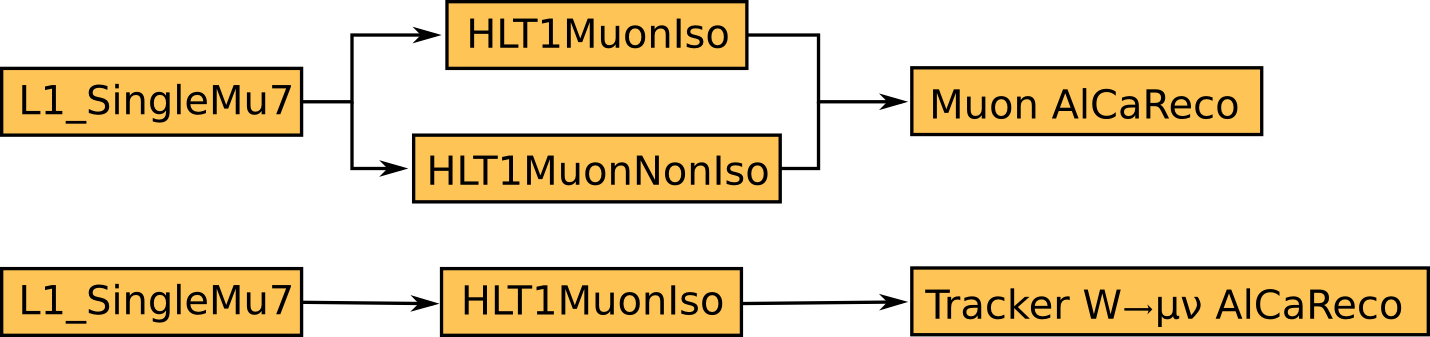
\includegraphics[height=2 cm]{path_standard.png}
\end{center}

\vspace{-0.25 cm}
\begin{itemize}
\item Based on conventional triggers
\item Validated and published to 2\_0\_X
\end{itemize}

\vfill Moreover, in early data, the roads defining ``L1\_SingleMu7''
can be widened (and in muon endcap, coincidence need not be required)

\vfill ``Open muon'' running would be useful in
\begin{itemize}
\item CRAFT (May--June)
\item Beam-halo from single-beam (June)
\item Low-luminosity collisions (July?)
\end{itemize}
%% \hspace{-0.83 cm} \textcolor{darkblue}{\Large Outline2}
\end{frame}

\begin{frame}
\frametitle{However\ldots}
\begin{itemize}
\item Nice to have a backup trigger that explicitly selects the kinds of events we're likely to see
\item Even in the long-term, we'll want non-I.P.\ tracks
\begin{itemize}
\item rate not tied to luminosity
\item improve convergence 
\end{itemize}
\end{itemize}

\begin{tabular}{p{0.4\linewidth} p{0.55\linewidth}}
\vspace{-0.5 cm} \begin{center}Example of a weak mode, poorly constrained by I.P.\ tracks alone\end{center} & 
\vspace{-0.5 cm} \begin{center}Simulated tracker alignment {\bf with} and \textcolor{red}{without} cosmics\end{center} \\
\vspace{-1.2 cm} \begin{center}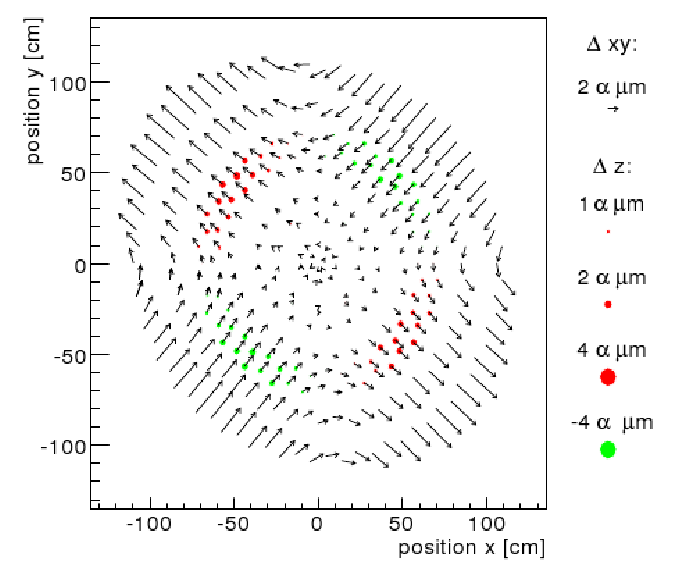
\includegraphics[height=4 cm]{weak_modes.png}\end{center} &
\vspace{-1.2 cm} \begin{center}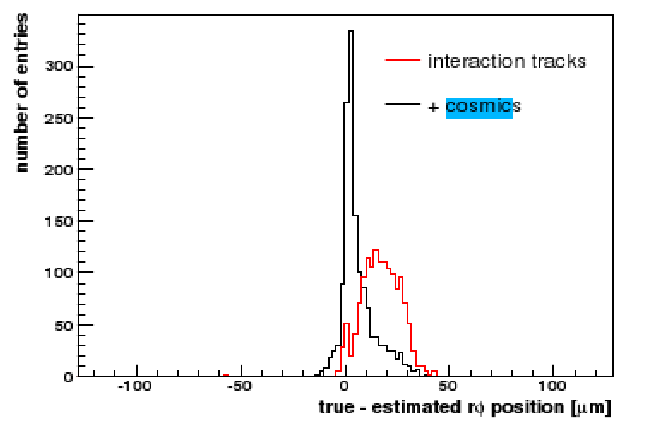
\includegraphics[height=4 cm]{addition_of_cosmics.png}\end{center} \\
\end{tabular}
\vspace{-0.5 cm}

\end{frame}

\begin{frame}
\frametitle{Sources of non-I.P.\ tracks}
Two categories:
\begin{itemize}
\item Cosmics
\begin{itemize}
\item best for barrels
\item tracker has expressed an interest
\item trigger from RBC
\end{itemize}
\end{itemize}

\begin{columns}
\column{0.5\linewidth}
\begin{itemize}
\item Beam-halo
\begin{itemize}
\item best for endcaps
\item tracker and muon systems are interested
\item disjoint intervals in radius, different \mbox{triggering mechanism\hspace{-1 cm}}
\begin{itemize}
\item Beam Scintillation Counters installed around tracker \hfill $\longrightarrow$
\item CSC beam-halo trigger from CSC trigger primatives
\end{itemize}
\end{itemize}
\end{itemize}

\column{0.5\linewidth}
\begin{center}
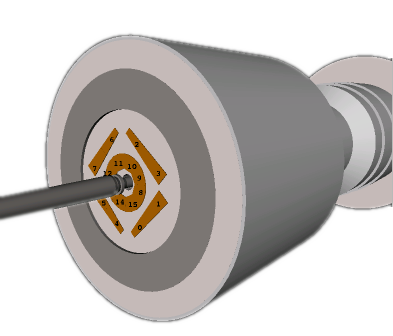
\includegraphics[width=\linewidth]{BSC_numbering-onshield.png}
\end{center}
\end{columns}

\end{frame}

\begin{frame}
\frametitle{Beam-halo in CSCs}
\begin{columns}
\column{0.4\linewidth}
\begin{itemize}
\item Steeply falling function of radius
\item Events in inner ring and outer ring are equally interesting
\end{itemize}

\vspace{1 cm}
\mbox{ }

\column{0.65\linewidth}
\hspace{-0.75 cm} 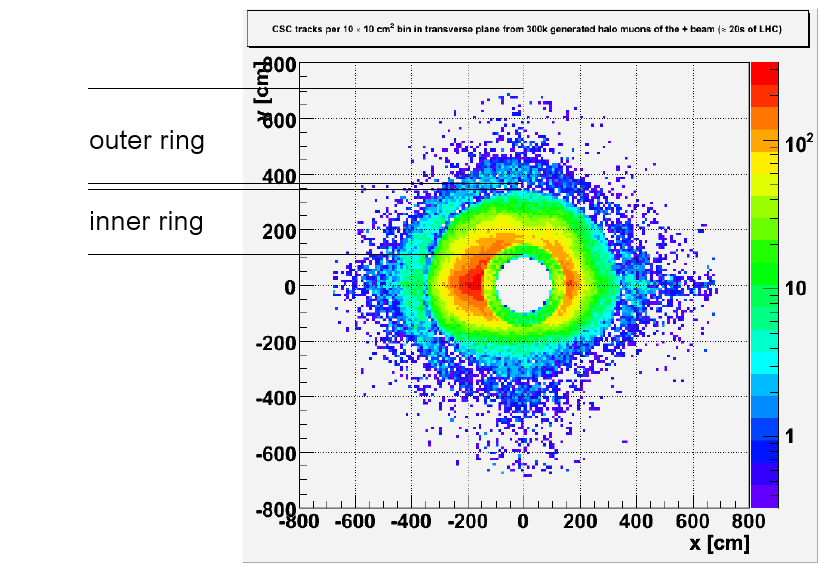
\includegraphics[width=\linewidth]{beam-halo.png}
\end{columns}

\vspace{-0.2 cm}
Two new HLT paths:
\begin{center}
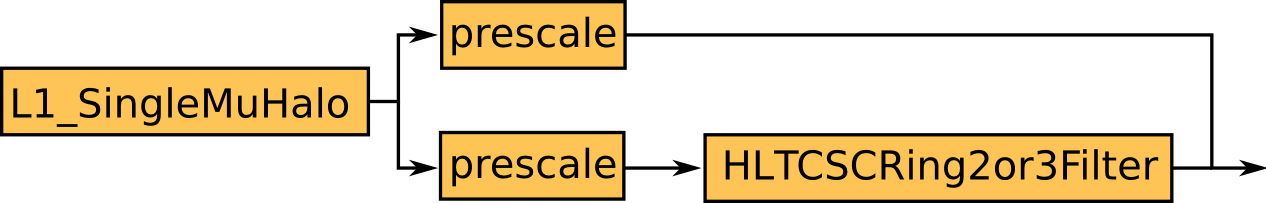
\includegraphics[height=1.3 cm]{path_beamhalo.png}
\end{center}

\begin{itemize}
\item HLTCSCRing2or3Filter selects at the level of RecHits
\begin{itemize}
\item 4/6 outer ring hits within 2~cm of each other (customizable)
\end{itemize}
\end{itemize}
\end{frame}

\begin{frame}
\frametitle{Beam-halo in CSC overlaps}
\begin{columns}
\column{0.7\linewidth}
\begin{itemize}
\item Tracks that intersect two neighboring chambers are particularly interesting
\begin{itemize}\setlength{\itemsep}{0.1 cm}
\item Get relative alignment of chambers without propagating track through iron
\item Design feature of CSCs, for alignment
\item Only about 5\% of the CSC area
\end{itemize}
\end{itemize}

\column{0.2\linewidth}
\vspace{0.5 cm}
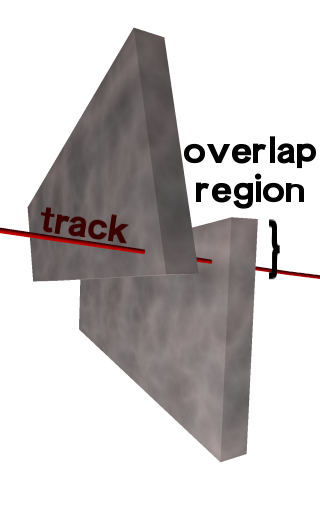
\includegraphics[width=\linewidth]{overlap.png}
\vspace{-0.5 cm}
\end{columns}

\vfill
Two new HLT paths:
\begin{center}
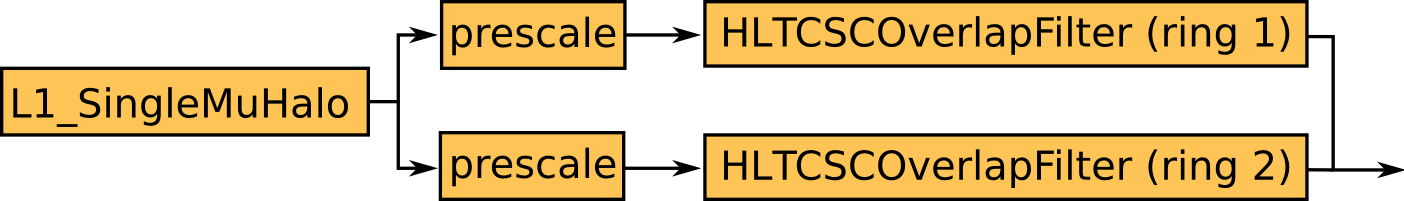
\includegraphics[height=1.3 cm]{path_beamhalo_overlap.png}
\end{center}

\vfill
\begin{itemize}
\item HLTCSCOverlapFilter selects at the level of RecHits
\begin{itemize}
\item 4/6 hits in each neighboring chamber within \mbox{2~cm (customizable)\hspace{-1 cm}}
\item Tuned in 10k MC
\end{itemize}
\end{itemize}
\end{frame}

\begin{frame}
\frametitle{Beam-halo in the tracker}

\begin{center}
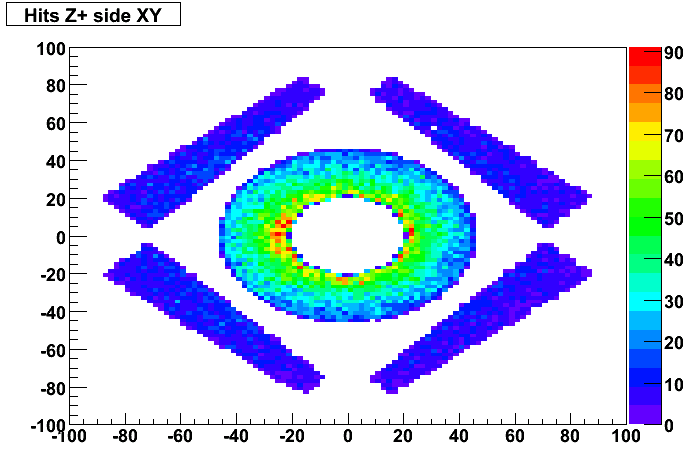
\includegraphics[width=0.6\linewidth]{XYpHalo.png}
\end{center}

\vspace{-0.5 cm}
\begin{itemize}
\item Two L1 bits, one for forward, one for backward
\item Rate is asymmetric: beam-halo from Sal\`eve $\gg$ from Jura
\item L1 indexes are unknown, currently filled with placeholders \\ \hfill (``1'' and ``2'')
\end{itemize}

\vspace{-0.3 cm}
Two new HLT paths:
\begin{center}
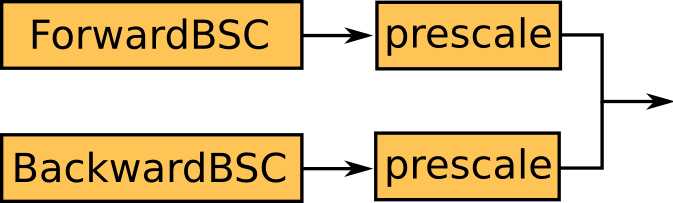
\includegraphics[height=1.3 cm]{path_tracker_beamhalo.png}
\end{center}

\end{frame}

\begin{frame}
\frametitle{Cosmic rays in the tracker}

\begin{itemize}
\item In the future, we'll want to select for pointing into the tracker
\item Currently, just pushes through the L1 bit
\item L1 index is unknown, currently filled with placeholder (``0'')
\end{itemize}

\vfill
One new HLT path:

\vspace{-0.5 cm}
\begin{center}
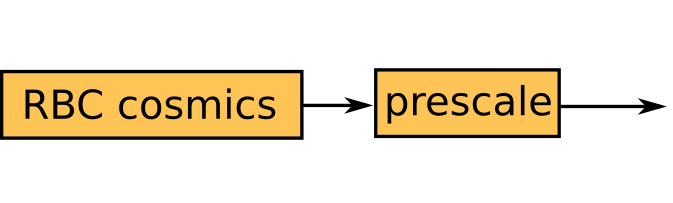
\includegraphics[height=1.3 cm]{path_tracker_cosmics.png}
\end{center}

\vfill
\hspace{-0.83 cm} \textcolor{darkblue}{\Large Configuration files in HLTrigger/special/data}

\vspace{0.1 cm}
\begin{itemize}\setlength{\itemsep}{0.2 cm}
\item Tagged with V00-01-54, but not yet published
\item Want to publish for 2\_0\_0, with ``CandHLT'' entries in HLTrigger/Configuration/data/main/Special.cff
\item Future corrections to L1 indexes and prescales are bug-fixes
\item All C++ code has been tested and tuned in MC
\end{itemize}

\end{frame}

\begin{frame}
\frametitle{Conclusions}
\begin{itemize}\setlength{\itemsep}{0.4 cm}
\item Most alignment tracks collected the same way as \mbox{physics muons\hspace{-1 cm}}
\item Technical triggers collect non-collisions muons for extra rate and non-I.P.\ pointing
\item 7 new HLT paths covering 4 use-cases
\item We want to publish these to 2\_0\_0 so that they won't be
rejected as ``new features'' in the future
\item Still need to finalize L1 bits, some haven't been assigned
\item Clearinghouse for alignment technical trigger information:
{\tt \scriptsize \textcolor{blue}{\mbox{\url{https://twiki.cern.ch/twiki/bin/view/CMS/TechnicalTriggersRequirements}}}}
\end{itemize}
\label{numpages}
\end{frame}

\end{document}
